% Created 2023-07-10 Mon 13:19
% Intended LaTeX compiler: pdflatex
\documentclass[11pt]{article}
\usepackage[utf8]{inputenc}
\usepackage[T1]{fontenc}
\usepackage{graphicx}
\usepackage{grffile}
\usepackage{longtable}
\usepackage{wrapfig}
\usepackage{rotating}
\usepackage[normalem]{ulem}
\usepackage{amsmath}
\usepackage{textcomp}
\usepackage{amssymb}
\usepackage{capt-of}
\usepackage{hyperref}
\author{Filipa  Calado}
\date{\today}
\title{}
\hypersetup{
 pdfauthor={Filipa  Calado},
 pdftitle={},
 pdfkeywords={},
 pdfsubject={},
 pdfcreator={Emacs 26.2 (Org mode 9.1.9)}, 
 pdflang={English}}
\begin{document}

\tableofcontents

\section{"'A Melon, an Emerald, a Fox in the Snow': Quantifying Gender in Virginia Woolf's \emph{Orlando: A Biography}"}
\label{sec:orgea40713}

\subsection{Abstract}
\label{sec:org832c732}

This chapter explores how the analysis of gender in text might
leverage gender theory to create a distant reading
methodology. Critiquing quantitative methods in Literary Studies that
perpetuate assumptions about gender as binary, this paper explores an
experimental approach that deconstructs social categories. It proposes
its own method for text analysis by drawing connections between
computer programming and gender theory. First, it delves into python
programming, focusing on the principle of iteration that drives
cleaning and regularizing tasks, as well as the transformation of
words into numerical representations for quantitative processing, with
the goal of bringing out the iterative quality of working with python
code. It then moves to Judith Butler’s concept of gender
performativity, which posits how gender expression might subvert
traditional social structures through repeatedly “performing” gender
constraints in ways that deviate from the norm. Taking this shared
quality of iteration between python and gender, it proposes a text
analysis methodology that interweaves, or iterates through, distant
and close reading. It then concludes by considering the limitations of
this method, which poses gender as a discursive phenomenon, and its
place within a larger trajectory of Gender Studies since Butler's text
inaugurating the field.

\subsection{Introduction}
\label{sec:org496aaaf}

The novel \emph{Orlando: A Biography} (1928), by Virginia Woolf, famously
opens with an assertive gender designation followed by an immediate
qualification: “He-for there could be no doubt of his sex, though the
fashion of the time did something to disguise it—was in the act of
slicing at the head of a Moor which swung from the rafters” (11). When
performing quantitative text analysis on this text, a fictional
biography of a 16th-century English nobleman who undergoes a sex
change, the standard tasks of “pre-processing” text evacuate the ways
that gender is unsettled in this sentence. In order to computationally
analyze a text, a process known which involves calculating and
visualizing textual patterns, the text must first be transformed into
a computable format. This task of pre-processing (also called
“cleaning” or “normalizing”) strips the original text of capitalized
words, punctuation, “stop words” (such as articles and prepositions),
and inflections in word endings, all of which are deemed to be
semantically minor, in order to make the text amenable to quantitative
analysis. Afterward, the following list of computable words, or
“tokens,” remain in the first sentence:
\begin{quote}
‘could’, ‘doubt’, ‘sex’, ‘though’, ‘fashion’, ‘time’, ‘something’,
‘disguise’, ‘act’, ‘slicing’, ‘head’, ‘moor’, ‘swung’, ‘rafter’.
\end{quote}
Cleaning this text not only strips it of its pronouns, including the
gender assertion in the first word, “He.” It also cuts the em dash
immediately following this "He," which signals the entrance of a
narrator that layers this assertion with conspicuous certitude: "—for
there could be no doubt of his sex…."

This chapter examines how quantitative text analysis works with
gender, using Woolf's \emph{Orlando} as a test case. Text analysis borrows
from natural language processing methods to do analyses like topic
modelling and sentiment analysis and machine learning methods like
logistic regression and word embeddings (discussed below), which
involves counting, classifying, and predicting textual
patterns. Though these methods differ in important ways, they share a
faith in using the speed of computation, which can process very
precise elements like word frequency or syntactic patterns, to analyze
large collections of textual data.

\subsection{The Fantasy of the Falsifiable}
\label{sec:orgcfb2be8}
Because computers can process hundreds of texts at a time, "reading"
at much faster rates than humans, attract critics who are interested
in the problem of scale in studying literary history. Critics like
Franco Moretti, Matthew Jockers, Ted Underwood, among others who pose
ambitious questions about literary history, led the development of
"distant reading" within Literary Studies. Moretti, who is largely
responsible for popularizing the practice of "distant reading" in
English Studies contexts, explores how social and economic forces
impacts literary form in the development of the modern novel. He
explains that the process of quantification involves steps that reduce
or abstract textual elements into computable form in ways that open
the potential for analysis: "fewer elements, hence a sharper sense of
their overall interconnection" (\emph{Graphs} 1). 

While critiques of Moretti abound (see Lauren F. Klein, "Distant
Reading After Moretti"), I want to focus on an early moment in his
career which anticipates a movement toward what I call "the fantasy of
the falsifiable." This moment, from Moretti's early essay "The Soul
and the Harpy" (1983), lays out the reasoning behind developing a new
methodological approach for literary criticism, which will eventually
flourish into "distant reading." Moretti in this essay betrays a deep
suspicion about the role of critical subjectivity in literary
analysis, which he calls "a sort of cultivated accompaniment to
reading" (21). By this, he means that the analytical practices of
contemporary literary critics, whose readings "revolve around concepts
such as ‘ambiguity’ and the like" will "always be pushed into
multiplying, rather than reducing, the obstacles every social science
encounters when it tries to give itself a testable foundation"
(22). Moretti likens the literary critic to a kind of Narcissus,
"whose only pleasure lay in contemplating his own reflection"
(14). The critic, he explains, focuses "on what has been lost and
become irretrievably unfamiliar, and which we can 're-familiarize'
only by doing such violence to it that we distort the objective,
material consistency of every work which it is the task of scientific
knowledge to reconstruct and 'salvage'" (14). Moretti's alternative
methodology grounds the critical process on a more solid foundation, a
"falsifiable criticism" that can "test" literary interpretations
(21). \emph{Falsifiable} here means that it must be contestable--one must
be able to imagine and carry out an alternative, ensuring the
"hypothesis" can be meaningfully tested--and falsifiable criticism
pursues answers that are "coherent, univocal, and complete" (21). This
kind of literary criticism would steadily progress toward irrefutable
knowledge. According to Moretti, "The day criticism gives up the
battle cry 'it is possible to interpret this element in the following
way', to replace it with the much more prosaic 'the following
interpretation is impossible for such and such a reason', it will have
taken a huge step forward on the road of methodological solidity"
(22).

As Moretti's falsifiable criticism eventually grows into "distant
reading," he streamlines his critical method into a recursive process
of posing hypotheses, collecting and assembling data, and making
inferences. The results are often unexpected, and sometimes bring
Moretti to reframe his hypotheses. This move relegates the literary
critic to the role of explaining results. For example, in “Style,
Inc.: Reflections on 7,000 Titles (British Novels, 1740-1850),”
Moretti plots book titles on a series of graphs in order to explore
how market forces influence the size and content of the titles. He
finds that titles are quite sensitive to the market: "As the market
expands, titles contract; as they do that, they learn to compress
meaning; and as they do that, they develop special ‘signals’ to place
books in the right market niche” (204). However, a closer look at his
language betrays the extent to which he makes interpretative moves at
every step:
\begin{quote}
in what follows, I focus on three moments of this history: first, I
\emph{describe} a major metamorphosis of eighteenth-century titles, and
\emph{try to explain} its causes; next, I \emph{suggest} how a new type of title
that emerged around 1800 may have changed what readers expected of
novels; and finally, I \emph{make a little attempt} at quantitative
stylistics, \emph{examining} some strategies by which titles point to
specific genres. Three sections, three pieces in the large puzzle of
the literary field. (181-2; emphasis mine)
\end{quote}
Moretti’s word choices here diminish the subjective work of critical
analysis--he \emph{describe[s]}, \emph{suggest[s]}, \emph{examin[es]}, etc. As
Stephen Ramsay points out, this language presents the literary
critic's work as an objective description of unproblematic reality, as
if his conclusions are supplementary to the graphs and other
visualizations. According to Ramsay, Moretti operates as if “data is
presented to us\ldots{} not as something that is also in need of
interpretation” (\emph{Reading Machines} 5). The computer's ability to
quantify textual data emboldens Moretti toward making seemingly
objective claims about literary history, all the while diminishing his
role as in analysis.

Ironically, the faith in the falsifiable gets its strongest expression
in a famous detraction by Nan Z. Da, published in the \emph{Journal for
Cultural Analytics}. Da argues that quantitative methods, which trade
"speed for accuracy, and coverage for nuance," reveal a "fundamental
mismatch betwen the statistical tools that are used and the objects to
which they are applied," (620, 601). Da emphasizes her point with an
experiment in "topic modeling," a deep learning method that generates
a number of "topics," or keywords, from large collections of text. Da
attempts to verify the results of a topic modelling experiment by
replicating the process on her own machine, a replication which
fails. She concludes that, "if the method were effective, someone with
comparable training should be able to use the same parameters to get
basically the same results" (628-629). As Ben Schmidt points out,
however, Da in fact uses different parameters and software to run her
experiments, which explains her results. His critique points out that
Da, in disqualifying quantitative methods for literary studies,
reinforces its role in positivist inquiry: "Far \emph{more} than anyone
I’ve seen in any humanities article, she asserts that scientists do
something arcane, powerful, and true.\footnote{For a more thorough critique of Da's aims and methodology in
this article, please see Ben Schmidt's "A computational critique of a
computational critique of computational critique,"} Despite their vastly
different views on the role of quantitative methods for studying
literature, Da and Moretti align on the value that they place on the
computer as a tool for a falsifiable kind of inquiry.

As Ted Underwood points out, "Both sides seem to be restating the
twentieth-century consensus that numbers are useful for measuring
objective facts but not for interpreting perspectival differences"
("Machine Learning" 93). Contrasting these approaches, Underwood uses
quantitative methods to offer "perspectival models" on literary
data. As Underwood himself explains, "Machine learning algorithms are
actually bad at being objective and rather good at absorbing human
perspectives implicit in the evidence used to train them" ("Machine
Learning and Human Perspective" 92). First, Underwood "trains" a
machine learning algorithm with sample data, for example, by marking
up character descriptions in text according to the gender of the
character being described. Then, this data is fed into the algorithm,
which "learns" which words are typically associated with women and
which words are typically associated with men. At the end of this
training process, the resulting "model" can be used to analyze gender
in new data by being given new text. Underwood describes this approach
as "perspectival modelling," because he can analyze the resulting
model only represents a single, rather than objective or universal,
perspective of the data. According to Dan Sinykin, this perspectival
method enables Underwood "to leverag[e] the human prejudices built
into modeling toward humanistic ends" (par. 4). For one of Underwood's
projects, which examines gender markers in novels, he uses a model
that predicts the the sex of a fictional character based on the words
associated with that character:
\begin{quote}
We represent each character by the adjectives that modify them, verbs
they govern and so on--excluding only words that explicitly name a
gendered role like \emph{boyhood} or \emph{wife}. Then, we present characters,
labeled with grammatical gender, to a learning algorithm. The
algorithm will learn what it means to be 'masculine' or 'feminine'
purely by observing what men and women actually do in stories. The
model produced by the algorithm can make predictions about other
characters, previously unseen. \emph{Distant Horizons} 115
\end{quote}
This particular model reveals that that, over time, gender roles in
novels become more flexible while the actual number of female
characters declines (\emph{Distant Horizons} 114). To explain this result,
Underwood conjectures that the practice of writing becomes more
commonly pursued as a male occupation in the middle of the 20th
century than it was previously (\emph{Distant Horizons} 137). This fact,
coupled with the tendency of men to write more about men than women,
explains why less women writing would led to a decline in female
characters.

However attentive to differences across male and female "perspective,"
Underwood's methodology nevertheless reinscribes the same binary that
it attempts to historicize. This becomes most clear in his study that
measures the "gendering of words used in characterization" ("Machine
Learning and Human Perspective" 95). Here, Underwood uses uses
logistic regression analysis, an entry-level machine learning
algorithm, to see whether words align with masculine or feminine
characters. This algorithm uses statistical reasoning to make
predictions on a scale of probability, from 1 to 0, for example,
between yes/no, pass/fail, win/lose, etc. In Underwood's case, the
probability is male/female (See Fig. 2). Here, Underwood admits that
"gender theorists will be frustrated by the binary structure of the
diagram" which "reduce[s] the complex reality of gender identification
to two public roles: men and women" ("Machine Learning" 98).

\begin{center}
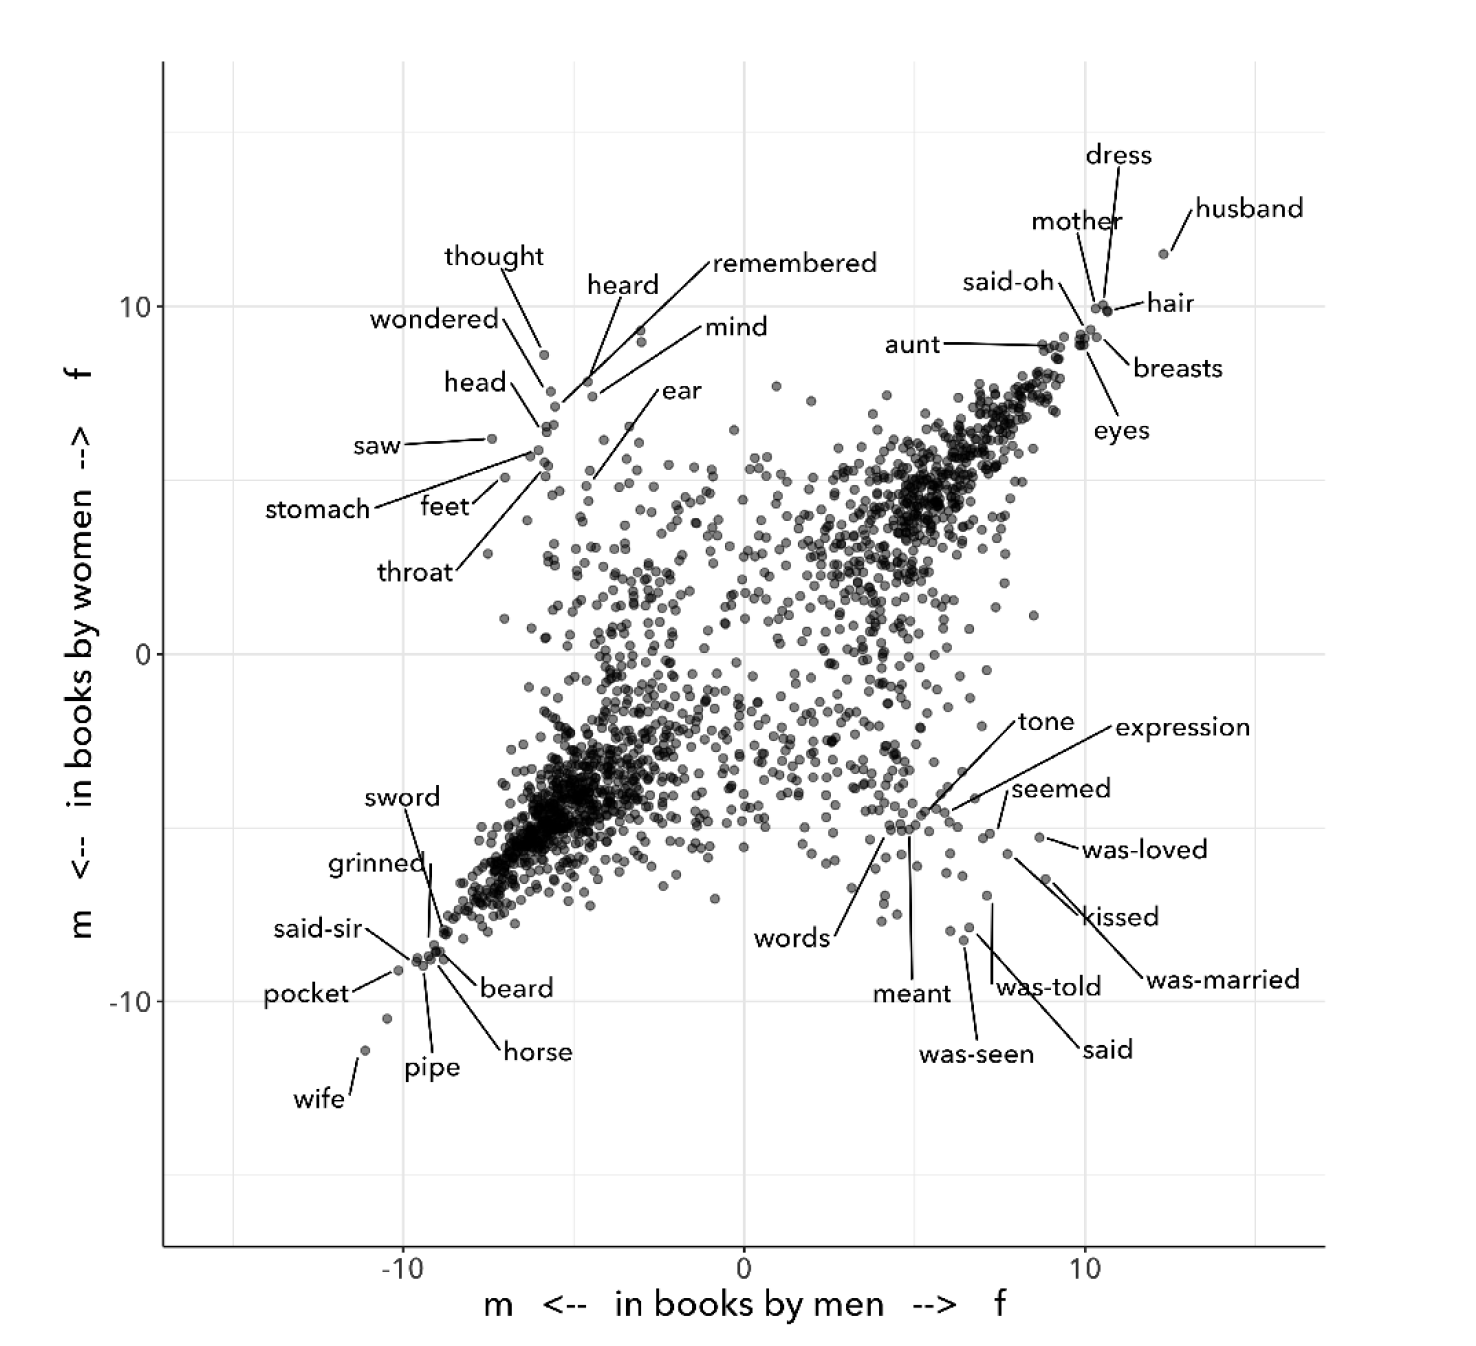
\includegraphics[width=.9\linewidth]{./img/Underwood.png}
\end{center} Caption: Underwood's logistic regression
model. The verticle axis visualizes the representation of words by
women, and the horizontal by men, with positive numbers signifying
overrepresentation of these terms. The terms on the left side of the
graph describe men, with the top-left corner and bottom-left corner
denoting books by male and female authors, respectively. The terms on
the right side of the graph describe women, with the top-right corner
and bottom-right corner denoting books by female and male authors,
respectively.


Collapsing of gender into a graph like this one brings to the surface
binary perspectives on gender markers across time. However, the
probablistic computations underlying this analysis reify gender as
either/or, in other words, as a binary opposition, a structural
tension that Underwood admits himself (\emph{Distant Horizons} 140). Here,
the concept of femininity is deliberately consolidated and computed
against that of masculinity, and the dual nature of the graph
constrains a reading of similarity or difference between the two terms
of analysis. Such is the purpose of Logistic Regression analysis which
collapses all possible answers to a yes or no probability. Asking a
machine to compute the conscription of gender as male or female for
the purpose of seeing how male and female roles in novels change over
time only \emph{reproduces} a model of gender that is "simple" enough to be
computed.

Without a doubt, reproducing conceptions of gender is useful for
historicizing gender identities and ideologies over time. In my view,
however, these approaches fail to harness the potential of both
computation and gender. It seems that the goal of establishing some
kind of knowledge about literary history, whether that be a "distant
horizon," or "the great unread," side-steps some of the more novel and
insightful processes a computer might undertake. Distant reading
methods might, for example, harness what Stephen Ramsay calls "the
objectivity of the machine," to destabilize the binary, readings that
are inescapably partial and speculative(x). Drawing from the
deformative critical methods of Jerome McGann and Lisa Samuels, Ramsay
proposes that researchers harness the enabling constraints of
computation to "unleash the potentialities" of the text, offering
opportunities for new readings (33).

Resisting the temptations of falsifiable criticism, work by critics
like Susan Brown and Laura Mandell apply distant reading methods
toward deconstructing gender as a historical concept. In their
introduction to \emph{The Journal for Cultural Analytics}'s "Identity
Issue," Brown and Mandell situate feminist debates around identity
politics as a necessary context for understanding how computational
processes engage gender identity. They explain that, "The goal is to
acknowledge the subjective effects of belonging to an identity
constituted historically through oppression without believing that the
identity itself exists independently from historical conditions"
(Mandell and Brown 6). In other words, because identity labels are
historically constructed, the computer can be used to study this
construction as a historical phenomena. Crucially, this position
places computational methods within a discursive frame, aligning it
with debates from post-structuralist feminist theory that explore and
provoke the representative capacities of language. In other words, the
computer can become a tool, not for verifying/reifying what we know,
but for exploring how language constructs (and can deconstruct)
categories.

In another project, Mandell uses distant reading to deconstruct what
she calls the "M/F binary." In her critique of distant reading
methods, Mandell illustrates how the study of gender often reifies
gender stereotypes, by "presenting conclusions about 'male' and
'female' modes of thinking and writing as if the M/F terms were simple
pointers to an unproblematic reality, transparently referential and
not discursively constituted" (par. 5). Mandell's examination
marshalls key findings from feminist theory, drawing from Judith
Butler, among others, to assert that gender is a socially constituted
category which is "constructed both by the measurer and the measured"
(par. 38). Computation offers, in Mandell's words, "parallax, multiple
perspectives for viewing a very complex reality” (par. 38). To
deconstruct gender, Mandell turns to genre, another category which
will allow scholars to see the reductive constitution of categories
generally. Here, Mandell uses the popular stylometry measurement,
"Burrow's Delta," which visualizes the "distance" between writing
styles by creating branches (or "deltas") between different texts. Her
experiment finds that the stylistic qualities of a female writer, Mary
Wollenstonecraft, shares with those of comparable male writers:
"Wollstonecraft’s sentimental anti-Jacobin novels most resemble
[William] Godwin’s sentimental anti-Jacobin novels\ldots{} whereas her
essays most resemble [Samuel] Johnson’s writings" (par. 29). By
drawing gender into conversation with genre, Mandell can "break the
strength of the signal," creating categories such as "'men writing as
men,' 'women writing as women,' 'women writing as men,' 'men writing
as women,' 'unspecified (anonymous) writing as men,'" and so on
(par. 35).

Just as quantification can be harnessed to deonstruct the M/F binary,
so it can deconstruct what Edwin Roland and Richard Jean So describe
as "the machine's initial binary understanding of race" (68). Roland
and So deconstruct racial categories by experimenting with an
algorithm that evaluates whether an author is white or black based on
diction. Analyzing a large corpora of novels by white and black
authors, they find that, black authors generally display more varied
vocabulary than white authors (66). From this they infer that white
authorship, as a category, only coheres against the variance of black
authorship. Whiteness, in other words, \emph{depends} on the
characterization of blackness.\footnote{Tie this relationship on the white/black binary to Eve
Sedgwick's points about binaries containing an oppostional dynamic in
which the subordinated term props up the dominant term.}

This quantitative exercise, rather than draw So and Roland toward
making general conclusions about race and authorship, points them
toward a peculiarity in the results: that the algorithm wrongly
categorizes James Baldwin's novel \emph{Giovanni's Room} (1956) as being
written by a white author. Apparently, the computer reads Baldwin's
use of the term "appalled" as proof of white authorsip. Going back to
the text, So and Roland discover that this term occurs only once, in
the early scene where David (the narrator) describes his strained
relationship to his father: "I did not want to be his buddy. I wanted
to be his son. What passed between us as masculine candor exhausted
and \emph{appalled} me" (my emphasis; Rpt. in So and Roland 71). Noting the
connotations of whiteness in "appalled," which has the middle French
root, "apalir," meaning "to grow pale," So and Roland insightfully
conclude that this term indexes an intersection of gender with race:
"the moment David develops a troubled relationship to normative
masculinity [as] also the moment he becomes 'white'" (71). The
computer's misclassification, as they point out, reinforces this
text's notorious elision of explicit references to race, whereby
racial markers are displaced in favor of an implicit whiteness, as
critics have observed in the scholarship on this novel. Taking the
computer's mistake as a starting point, So and Roland's analysis thus
contributes to the ongoing debate about the complex relationship
between race and sexuality in the novel.

Rather than "fixing their results as stereotype," as Mandell
describes, the computer enables researchers to "animate numerical
processes" (Mandell par. 7). In direct opposition to the "falsifiable"
position, computational error becomes a starting point for
analysis. Because race is a social construct, and machines only impute
meaning that is encoded into them, So and Roland reason that machines
are be ideal instruments for studying the construction of race
(60). The machine errors surface a yet unexplored fulcrum around which
the binary of race turns, that of queerness:f
\begin{quote}
Our reading’s destabilization of the machine’s logic of white and
black arises directly from the novel’s expression of queerness. By
queering the machine’s color line, Baldwin’s novel challenges our
initial classifications of the novels as white or black, which had
necessarily effaced a more sophisticated, intersectional view of
social identity. In their current form, our data and model are not
robust enough to handle this kind of intersectionality. 72
\end{quote}
Like Mandell, So and Roland move beyond historicizing gender. In this
case, a single computational error opens a site for more daring leaps
of speculation about how whiteness gestures toward a troubled
understanding of sexuality, where queerness operates as an
articulation (both structurally and semantically) of race.

\subsection{Iteration}
\label{sec:org9c2298d}
As Mandell points out, both gender and genre "are\ldots{} highly
imitatable," so that "anyone can adopt gendered modes of behavior,
just as anyone can write in genres stereotypically labeled M/F"
(par. 30). While this interpretation of gender performativity echoes a
common misunderstanding which Butler is careful to explain in her
writings since \emph{Gender Trouble}, gender performativity does offer a
useful heuristic for quantitative text analysis. In what follows, I
bring gender theory and quantitative processes into alignment, tracing
the process of "cleaning" text, popular text analysis tasks, through
"deep learning" methods for encoding semantic information. As I will
demonstrate, Butler's theory has a lot to lend to the study of
computational text analysis.

First, the common misreading of Butler's theory is that gender
performativity denotes an act or series of acts that can be imitated
at will, to be put on and off like clothing. As Butler emphasizes in
her follow up book, \emph{Bodies that Matter: on the Discursive Limits of
Sex} (1996), performativity is compulsory and habitual, a process that
precedes and constitutes the subject.\footnote{In her groundbreaking book, \emph{Gender Trouble: Feminism and the
Subversion of Identity} (1990), Judith Butler famously disrupts two
essentialist views of sex and gender in contemporary feminist thought:
first, that sex is biological while gender is constructed; and second,
the gender, as a construction, is a self-expression of the
subject. Because sex and gender are both constructions that exist
prior to identity. According to Butler, there is no such thing as a
subject that exists prior to gender expression, as a subject only
comes into being by participating in a gender norm.} Butler explains that
gender is a mechanism that allows the subject to emerge: "construction
is neither a subject nor its act, but a process of reiteration by
which both 'subjects' and 'acts' come to appear at all" (\emph{Bodies}
xviii). This process of "reiteration" is fully delineated in her
concept of "performative citation," whereby what is experienced as the
physical body, its boundaries and its sexuality, only materialize
through the repetition, the "citation," of gender norms, whereby each
act signals an authorizing norm.

Common critiques of Butler point out the limits of this theory for
posing gender and sexuality as discursive.\footnote{Another popular critique comes from Political Philosophy, and
concerns a logical inconsitency in the way that Butler theorizes
subjectivity. If the resistance to signification comes from outside
the cycle of signification, from where does that external resistance
emerge? Does it not imply a pre-discursive identity or at least desire
for resistance? Geoff Boucher writes that Butler locates the potential
for subversion "in a disembodied intentionality that appears to stand
outside of the culturally-scripted subject positions that the
individual occupies" (115). He aptly questions: "Who (or what) decides
'how to repeat'? On what basis is the decision to subvert power made?"
(119).} Jay Prosser, coming
from the field of Trans Studies, problematizes Butler's
"deliteralization of sex," a critique that he applies to Queer Studies
more generally. Prosser explains that because Butler's analysis
attends to performativity as a discursive phenomenon, it elides the
real-world concerns of the body's materiality. Prosser offers the
example of Butler's reading of \emph{Paris Is Burning}'s Venus Xtravaganza
who, Butler argues, occupies a space of transgression due to her
inability to attain her sex change. According to Butler, a sex change
that would "make [her]self complete" would also fulfill the desire for
a masculine body would reinscribe heterosexual hegemony (45). Prosser
points out that this reading fails to reckon with the material body
and its precarious existence, as Venus's death illustrates
(55). Butler's "metaphorization of the transgender body" demonstrates
one crucial way that Queer Theory has subsumed, without fully
accounting for, transgressive desires in cross-gendered
identifications. This thread of discursivity and its implications is
picked up in the conclusion, where it instigates the next move within
a larger trajectory of Queer Studies presented in this dissertation.

To understand the constraints of performativity as a discursive
phenomenon, it is helpful to situate Butler's work within the context
of second-wave feminism and its post-structural approach toward gender
binaries. Here, Butler draws from the work of feminist theorist Luce
Irigaray, who asserts that influential Western thinkers, like Plato,
Aristotle, and Freud, for example, have defined women and feminity "on
the basis of masculine parameters" (Irigaray, \emph{The Sex Which Is Not
One} 23).\footnote{Irigaray's critique of gender undermines what Jacques Derrida
famously defines as "phallogocentrism," the idea that man, symbolized
by the phallus, is the center and focus of knowledge.} The resulting binaries that associate "woman" with
"matter" (such as "rationality/emotion" and "mind/body"), and set it
subordinate to male "form," effectively erase the possibility of
representing woman at all. Rather, the binary actually "\emph{produces} the
feminine as that which must be excluded for that [gender] economy to
operate" (10; my emphasis). The produced "domesticated" feminine term
contrasts the excessive feminine which cannot be expressed within the
terms of the binary (13). This "necessary outside" of the excluded
feminine, which is in fact is the enabling condition of the binary in
the first place, creates a "field of disruptive possibilities"
(13). However, this "unspeakable" element cannot be invoked directly,
"through the figures that philosophy provides," without subscribing
itself to the ruling structure (12). Butler illustrates this quandry
with a hypothetical: "how can one read a text for what does \emph{not}
appear within its own terms, but which nevertheless constitutes the
illegible conditions of its own legibility?" (11). For Butler, this
question--how to express what is not there, what is refused by the
system of the visible--will guide her theory of gender subversion.

For Butler, theorizing subversion begins by positing the origin of
signification, which leads her to the performative quality of
language. Butler wonders, "Can language simply refer to materiality,
or is language also the very condition under which materiality may be
said to appear?" (6). Butler finds that, in order to refer to a body,
language must first assume a body. Therefore, she reasons, the
signification of the body actually creates the body which it appears
to reference: "signification produces as an \emph{effect} of its own
procedure the very body that it nevertheless and simultaneously claims
to discover as that which \emph{precedes} its own action" (emphasis
original; 6). This reasoning leads Bulter to a major realization: "the
mimetic or representational status of language\ldots{}. is not mimetic at
all. On the contrary, it is productive, constitutive, one might even
argue performative" (6). This point, that language produces the
reality that it seems to merely reference, means that subjects are
always interpellated, and in fact brought into subjectivity, by a
discourse prior to their their participation in it.

However, within this regulatory structure, this significatory circle,
lies the possibility of resistance, the possibility of \emph{resignifying}
meaning. Because language transcends a merely representative function,
because it works to \emph{produce} meaning, language can be resignified
toward subversive usages by "citing" what Bulter calls the
"repudiated" meaning implied by signification. Butler offers the
famous example in the resignification of the term "queer," which has
been transformed from a term of abjection to one of
empowerment. "Queer" achieves this resignification by harnessing its
own repudiation, which is an implied but "disavowed abjection [that]
will threaten to expose the self-grounding presumptions of the sexed
subject" (3). In other words, each time the term "queer" is used, it
draws from that abjection which is repudiated in every identification
with heterosexuality. Butler proposes that one "cite" this repudiation
as a resource for resignification: "to consider this threat and
disruption\ldots{} as a critical resource in the struggle to articulate the
very terms of symbolic legitimacy and intelligibility" (3). Here, the
concept "citation" indicates an act of signification that draws from
the authorizing power. By citing the repudiated meaning, the term
"queer" "resignifyi[es] the abjection of homosexuality into defiance
and legitimacy" (xxviii). The resignification works because this
"performative citation" takes on the repudiation as its signification.

Here, repetition is key, enabling the introduction of what is external
to the binary into the system. Irigaray achieves this resistance by
performing the phallogocentric language of the thinkers that she
criticizes. Butler explains, "she mimes philosophy\ldots{} and, in the
mime, takes on a language that effectively cannot belong to her"
(12). Irigaray uses performative citation as a strategy of undermining
authority through repetition: "She cites Plato again and again, but
the citations expose precisely what is excluded from them, and seek to
show and to reintroduce the excluded into the system itself"
(18). Through repetition, Irigaray displaces the logic of
phallogocentrism, introducing something external to the system while
remaining within its terminology. Butler narrates what she imagines to
be Irigaray's thought process on resiting this logic:
\begin{quote}
I will not be a poor copy in your system, but I will resemble you
nevertheless by miming the textual passages through which you
construct your system and showing that what cannot enter it is already
inside it (as its necessary outside), and I will mime and repeat the
gestures of your operation until this emergence of the outside within
the system calls into question its systematic closure and its
pretension to be self-grounding" (18).
\end{quote}
Here, deception emerges from resembland, and insubordination through
subservience. The key is iteration, a continual activity, the miming
of the authorizing norm, which displaces it by introducing what is
outside the logic of phallogocentrism. In the next section, I examine
how this process of iteration, drawing from abjection, engages with
text analysis.

Recalling the opening example in this chapter, the process of
preparing or "cleaning" a text for text analyis always requires a
reduction of data in which some semantic value has escaped. In this
example, the first sentence of Woolf's novel, \emph{Orlando}: "He–for there
could be no doubt of his sex, though the fashion of the time did
something to disguise it—-was in the act of slicing at the head of a
Moor which swung from the rafters" (11), is striped of pronouns and
punctuation which has the effect of surpressing the gender
qualification. After processing, the following words remain:

\begin{quote}
‘could’, ‘doubt’, ‘sex’, ‘though’, ‘fashion’, ‘time’, ‘something’,
‘disguise’, ‘act’, ‘slicing’, ‘head’, ‘moor’, ‘swung’, ‘rafter’. 
\end{quote}

In what follows, I deconstruct the cleaning and text analysis
processes to surface how computational syntax evokes the quality of
iteration that constrains gender performativity. 

To do common text analysis tasks, many distant reading projects use
the Python programming language, which offers a number of custom
"libraries," or collections of code for specific tasks, such as the
Natural Language ToolKit (NLTK). This library contains useful
computational "methods" and "functions" that count, categorize, and
visualize textual patterns.

Before moving forward with NLTK and text cleaning, it is necessary to
explain how Python handles text-based data. When analyzing text,
Python works with data in the form of words, or \texttt{strings}, contained
within groupings called \texttt{lists}. Then, Python \emph{iterates} through the
list, to perform a task to each item in the list. The expresion for
this functionality, called the \texttt{for loop}, repeats a single action to
each item, like a \texttt{string}, over a collection of data, like a
\texttt{list}. Also known as "looping" or "iterating" through the \texttt{list}, the
instructions specify some action to each item in the \texttt{list}. The
syntax of the for loop contains two lines: the first defines the data
to be iterated and the second contains an instruction. In the code
below, for example, the expression \texttt{for word in sentence:} specifies
each \texttt{string} in a \texttt{list}, and the second line \texttt{print(word)} instructs
the computer to display each \texttt{string}, one by one, in the
sentence. Essentially, this loop will go through each item in the data
and it will display that data:

\begin{SOURCE}
sentence = ['He', '--', 'for', 'there', 'could', 'be', 'no', 'doubt',
'of', 'his', 'sex', ',', 'though', 'the', 'fashion', 'of', 'the',
'time','did', 'something', 'to', 'disguise', 'it', '--', 'was', 'in',
'the', 'act', 'of', 'slicing', 'at', 'the', 'head', 'of', 'a',
'Moor','which', 'swung', 'from', 'the', 'rafters']

for word in sentence:
    print(word)

['He',
 '--',
 'for',
 'there',
 'could',
 'be',
 'no',
 'doubt',
 'of',
 'his',
 'sex',
 ',',
 'though',
 'the',
 'fashion',
 'of',
 'the',
 'time',
 'did',
 'something',
 'to',
 'disguise',
 'it',
 '--',
 'was',
 'in',
 'the',
 'act',
 'of',
 'slicing',
 'at',
 'the',
 'head',
 'of',
 'a',
 'Moor',
 'which',
 'swung',
 'from',
 'the',
 'rafters']
\end{SOURCE}

These kinds of iterative computations are a core component of working
with text. At a very basic level, much of text analysis consists of
iterating over bits of text and doing something to each word in the
text, performing actions that will prepare and standardize the text
for analysis. In preprocessing text, such main tasks include
tokenizing, cleaning, and regularizing, which help to eliminate pieces
of text that will skew the results of analysis due to their high
frequency and low semantic value. Tokenizing the text means separating
the text into workable units, or \texttt{tokens}, that are easier to clean
and regularize. Once the text is tokenized, it can be stripped of
capital letters, punctuation, and what are called "stop words," which
consist of prepositions, articles, and related terms, such as "he,"
"for," "there," "be," "of," "the," and "did" in the above example. The
following code block loops through the text to remove punctuation and
capital letters:

\begin{SOURCE}
normalized = []

for word in full-text:

if word.isalpha():

normalized.append(word.lower())
\end{SOURCE}

Here, it begins by creating an empty list, \texttt{normalized}, where
words will be dropped after filtering through them. The next line
begins the \texttt{for loop}, which iterates through each word in the
\texttt{full-text} list of words. The third line, an \texttt{if statement} creates
the condition specifying alphabetic characters (containing no numbers
or punctuation), and if the word fulfills that condition, then it
passes to the fourth line, which will add that word to the
\texttt{normalized} list. At the moment that this word is added to the
list, its letters will be transformed to lowercase format. The final
list, therefore, will contain words that are all lowercase and contain
no punctuation.

The next step involves removing stop words, then
stemming/lemmatizing. For this process, the \texttt{for loop} can be
compressed into a \texttt{list comprehension} format:

\begin{SOURCE}
no-stops = [word for word in normalized if word not in stops]
\end{SOURCE}

This expression takes each word in a list, in this case, \texttt{normalized},
and checks to see if that word is also contained within the list of
stop words in \texttt{stops}. If the word is \emph{not} a stop word, then it will
be added to a new list, \texttt{no\_stops}. Once this filtering is done, the
final list contains all lowercase words without punctuation or stop
words. For example:

\begin{SOURCE}
['could', 'doubt', 'sex', 'though', 'fashion', 'time', 'something',
'disguise', 'act', 'slicing','head', 'moor', 'swung', 'rafters']
\end{SOURCE}

After cleaning the text in this way, the next step involves stripping
the grammatical structure to get the word root. There are two options,
which differ in how much computational processing each requires. The
first of these processes, called "stemming", involves cutting off the
endings from the word. For example, "rafters" will be stripped to
"rafter." In the other process, called "lemmatizing," the computer
will look up each word, one by one, find its appropriate root, and
then revert to that root. Because this process requires verifying the
root for each word, it takes longer and is more computationally
intensive than stemming.

\begin{SOURCE}
clean = [WordNetLemmatizer.lemmatize(word, word) for word in no-stops]
\end{SOURCE}

These tasks of preprosessing text force words into existing boxes, so
to speak, in order to make them amenable to analysis. The effect of
this preprocessing therefore strips text of some of its semantic
meaning, which can be contained in capitalized words, rhythms of
language in stop words, inflections in word endings, and so on. This
is not to say that preprocessing ought to be avoided, but that the
researcher should be aware of how certain textual reductions have the
potential to affect meaning.

At this point, the text is ready for analysis. At the root of many
text analysis tasks are word frequencies which also includes the
frequency of words surrounding a given word. For example,
\texttt{concordance()} method returns the context, that is, the immediate
words surrounding the word "woman" from the text of \emph{Orlando}:

\begin{SOURCE}
alities which the old woman loved the more the mo

scarlet . For the old woman loved him . And the Q

les . The old bumboat woman , who was carrying he

h , whether boy 's or woman 's , for the loose tu

boy it must be -- no woman could skate with such

eadth off . She was a woman . Orlando stared ; tr

, until now ? An old woman , he answered , all s

and some old country woman hacking at the ice in

and pity the poor old woman who had no such natur

man 's beard and that woman 's skin ; of a rat th

the sight of the old woman hobbling over the ice

ght coming or the old woman or whatever it was , 

tainly not those of a woman bred in a cattle-shed

e world for a Cossack woman and a waste of snow -

erating . There was a woman in white laid upon a 
\end{SOURCE}

Building from the same concept as the \texttt{concordance()} method, another
method, called \texttt{similar()} calculates words which are used in similar
contexts as the target word. To compute the results of \texttt{similar()},
NLTK first takes the context of the term from \texttt{concordance()}, then it
searches the text for other terms which contain the same surrounding
words. The result for running \texttt{similar} on the word "woman" is the
following:

\begin{SOURCE}
man moment night boy word world child pen ship door one room window
light little lady table book queen king
\end{SOURCE}

By searching the text for words that appear \emph{similarly} to the chosen
word, this method reveals words that function in semantically similar
ways across the text. It is important to point out, however, that the
text itself does not impute meaning to the words. Rather, it can only
count words as "strings," that is, bits of data composed of
alphanumeric sequences. It takes the string "woman," takes notes of
all of the strings in proximity to "woman," and then searches the rest
of the text for \emph{other} strings that have similar proximities. This
method is based on counting frequencies of characters that occur near
each other.

Basic natural language processing tasks offered by libraries like NLTK
often lead to algorithmic and "deep learning" methods that work in
more sophisticated ways to count and analyze language. Many of these
methods use the concept of "word embeddings" to ascribe
machine-interpretable meaning to \texttt{strings}. Like \texttt{similar()} and
\texttt{concordance()}, word embeddings build off patterns of word similarity
based on context. Unlike the NLTK methods, however, word embeddings
encode a value to a given word based on its context. The value of any
given word is a numerical representation, actually a list of numerical
representations, known officially as a "word vector." A vector for a
single word, "woman," for example, will contain a list of numbers
which represent "woman." Specifically, each vector in this list
represents a similarity score between "woman" and a related word. As
numerical representations, these values enable quantitative processes
that can analyze the relationship between "woman" and other words. The
classic example for introducing the power of word embedding methods is
the formula, "King - Man + Woman = Queen" (Mikolev et al. 2). Here,
gender (between "Man" and "Woman") is isolated as a computable
component which enables one to derive the difference between "King"
and "Queen".

The vector which represents "woman" contains a list of numbers that
score "woman's" similarity to related words. Here, the word "woman" is
most closely associated to the word "child," with a similarity score,
or "weight," of .93, or 93\%, then with "mother," with its weight being
.92, then "father," which has a weight of .90.\footnote{The language model for this computation comes from
Word2Vec's "glove-twitter-25" dataset.} Below is a full
list of word vectors calculated as most similar to "woman":

\begin{SOURCE}
[('child', 0.9371739625930786),

('mother', 0.9214696884155273),

('whose', 0.9174973368644714),

('called', 0.9146499633789062),

('person', 0.9135538339614868),

('wife', 0.9088311195373535),

('being', 0.9037441611289978),

('father', 0.9028053283691406),

('guy', 0.9026350975036621),

('known', 0.8997253179550171)]
\end{SOURCE}

Commonly, word embeddings are organized into a "matrix," that is, a
tabular format"

\begin{center}
\begin{tabular}{lrrrrrrl}
Target Word & child & mother & whose & called & person & wife & \ldots{}\\
\hline
Woman & .937 & .921 & .917 & .915 & .914 & .909 & \ldots{}\\
\end{tabular}
\end{center}


Given this tabular representation, numerous mathematical operations
are possible using principles from statistics, linear algebra, and
calculusl, as well as "deep learning" methods, like neural networks,
in which the labels of the numerical representations do not matter. In
deep learning, the only thing that matters is the list of numbers
themeslves, which together represent the word. The word "woman,"
therefore, would be represented with the following vector: .937. .921,
.917, .915, .914, .909, and so on. Deep learning methods demonstrate
that, even when removing semantic labels, \emph{words are assigned meaning
by their relation to other words}. Even with each of these words
represented as a vector with the labels removed, the sexism of the
formula remains obvious: the woman is computed according to her
relation to a man.

\subsection{Queer Distant Reading}
\label{sec:org10e368d}
I now turn to Virginia Woolf's novel, \emph{Orlando: A Biography}. This
novel is ideal for a computational study of gender for two
reasons. First it is perhaps the most salient example of transgender
narrative in the modernist era. Second, as many critics have noted,
its characterisitic modernist experimentation with limits of language
work toward destabilizing gender norms.\footnote{Much of the scholarship on this text explores its resistance
against normative concepts of identity and gender. The experimental
use of language and narrative form creates a narrative that is
recalcitrant against coherent understandings of gender and
identity. Jane de Gay, Jill Channing, and Christy L. Burns, for
example, assert that Woolf deploys imaginative elements, magical
realism, and parody, respectively, to resist realism and narrative
expectations in her fictional biography. De Gay aligns Woolf's writing
with that of Walter Pater and Vernon Lee as a "feminist
historiography" that "rejected Victorian patriarchal metanarratives"
and instead "used the strategies of fiction to bring history alive and
make it live in the present" (de Gay 71). In a similar vein, Burns and
Channing both point out that Woolf uses fantastical elements, in the
former in the service of parody, and the latter as part of magical
realist writing, that disrupt expectations of plot and narrative to
challange the stability of gender and identity. Doubling down on the
role of langauge, some critics emphasize that the narration
purposefully obfuscates any resolution about concepts like gender,
identity, and even race and nationality. Victoria L. Smith asserts
that "The fantastic content in the novel is directly linked to the
undecidability/impossibility of the form of the novel and of the
protagonist" (58).} In what follows, I draw
from aspects of gender performativity to pursue an \emph{iterative} text
analysis based on the word embeddings of the gender markers, "woman"
and "man," of this text. I call this method "iterative" because it
moves between close and distant reading, what Andrew Piper calls
"bifocal" reading, in a way that iterates over the output of previous
computations. This method, as Piper explains, "no longer us[es] our
own judgments as benchmarks\ldots{} but explicitly construct[s] the context
through which something is seen as significant (and the means through
which significance is assessed)" (17). 


First, I begin with a list of terms computed similar to woman and man,
respectively, in the text. Unlike the word embeddings from my previous
section, which were trained on Twitter data, the language model here
is trained on Woolf's novel, and therefore reflect an understanding of
gender markers based on how words are used in this specific text.

The following are words associated with "woman":

\begin{SOURCE}
[('would', 0.5118660926818848),

('hand', 0.5049053430557251),

('night', 0.4855204224586487),

('though', 0.4815906882286072),

('way', 0.476143479347229),

('foot', 0.4528403580188751),

('orlando', 0.433744877576828),

('said', 0.43140658736228943),

('like', 0.41121190786361694),

('life', 0.4069981873035431)]
\end{SOURCE}

And the following are words associated with "man":

\begin{SOURCE}
[('would', 0.6174017786979675),

('orlando', 0.6018419861793518),

('night', 0.5755824446678162),

('way', 0.5710440874099731),

('great', 0.5492382645606995),

('long', 0.5454811453819275),

('could', 0.53724604845047),

('table', 0.5338666439056396),

('thus', 0.533319354057312),

('said', 0.5238105058670044)]
\end{SOURCE}

The lists reflect commonly used words, and appear somewhat similar,
sharing terms like "would," "orlando," "night," and "way." To get more
distinctive results for each gender, I modified the code to remove any
words with strong associations to the opposite gender. Recalling
Butler, this moves takes the \emph{repudiated} term, either "woman" or
"man," and feeds it back into formula. The results revealed more
distinctive words associated with each gender:

\begin{SOURCE}
> distinct\(_{\text{w}}\) = model.wv.most-similar(positive="woman", negative="man")

[('soft', 0.3692586421966553),

('named', 0.34212377667427063),

('sciatica', 0.3223450779914856),

('frilled', 0.3187992572784424),

('despaired', 0.31375786662101746),

('friend', 0.31238242983818054),

('delicious', 0.30853813886642456),

('winked', 0.30514153838157654),

('notion', 0.3047487139701843),

('seductiveness', 0.30290719866752625)]


> distinct\(_{\text{m}}\) = model.wv.most-similar(positive="man", negative="woman")

[('chequered', 0.4025157392024994),

('fact', 0.3394489586353302),

('denounced', 0.3346075117588043),

('house', 0.33423593640327454),

('curiosity', 0.33144116401672363),

('defend', 0.3284823000431061),

('dancing', 0.3282632827758789),

('marbling', 0.3184848427772522),

('cynosure', 0.3057470917701721),

('rather', 0.3024100363254547)]
\end{SOURCE}

At first glance, the top terms for each list appear to align with
existing conceptions of femininity and masculinity, such as "soft" for
"woman," and "chequered" for "man."  The rest of the terms also appear
to uphold a binary understanding of gender, with words like "frilled,"
"delicious," and "seductiveness," associated with "woman," and "fact,"
"defend," and "denounced" associated with "man."

Beyond these general patterns, however, the results complicate an easy
understanding of gender as binary. In what follows, I use some of
these words as starting points for close-reading analysis of the
text. I begin with unique words from both lists which, appearing only
once in the text, carry significant semantic weight in their relation
to gender. Then, I examine words that co-occur in certain passages of
the texts--moments which are provocatively indicative of the
relationship between gender and language in the text.

Interestingly, while the top term for the "woman" category, "soft," is
used 9 times throughout the text, the top term for the "man" category,
"chequered" is only used once, at the very beginning of the story,
when Orlando makes his entrance, stepping "the yellow pools chequered
by the floor" (Woolf 12). This moment is the first of many in which
the narrator casts doubt his credibility as a biographer, the
self-described "scribe." Soon after Orlando makes his appearance, the
narrator distinguishes his role as a biographer from that of the poet,
who works to embellish and exagerrate through figurative
language. However, the narrator's committment to straightforward and
solemn description soon unravels when he attempts to describe
Orlando's beauty. Here, the language swells to full-fledged
figuration:
\begin{quote}
Directly we glance at Orlando standing by the window, we must admit
that he had eyes like drenched violets, so large that the water seemed
to have brimmed in them and widened them; and a brow like the swelling
of a marble dome pressed between the two blank medallions which were
his temples. Directly we glance at eyes and forehead, thus do we
rhapsodize. Directly we glance at eyes and forehead, we have to admit
a thousand disagreeables which it is the aim of every good biographer
to ignore. 12-13
\end{quote}
Here, the narrator's evocative language undermines the pretense to
objectivity which he feels compelled to produce. This doubt grows into
a crisis of signification that occurs persistently throught the
novel. That the usage of "chequered" in this passage suggests that
gender may have something to do with this crisis.

The crisis of signification also occurs within Orlando's experience
itself. From the "woman" list, I take a term, "despaired" which, like
"chequered," occurs only once in the novel. It appears at a point when
Orlando, deep in a depression following his desertion by his first
love, Sasha, struggles to understand the role of figuration in
language: 
\begin{quote}
So then he tried saying the grass is green and the sky is blue and so
to propitiate the austere spirit of poetry whom still, though at a
great distance, he could not help reverencing. 'The sky is blue,' he
said, 'the grass is green.' Looking up, he saw that, on the contrary,
the sky is like the veils which a thousand Madonnas have let fall from
their hair; and the grass fleets and darkens like a flight of girls
fleeing the embraces of hairy satyrs from enchanted woods. 'Upon my
word,' he said (for he had fallen into the bad habit of speaking
aloud), 'I don't see that one's more true than another. Both are
utterly false.' And he \emph{despaired} of being able to solve the problem
of what poetry is and what truth is and fell into a deep
dejection. 75; emphasis mine
\end{quote}
Like the narrator from the previous passage, Orlando here interrogates
the truthfulness of figurative elements. First, he attempts plain
language, "the sky is blue", "the grass is green," but these prove
insufficient for describing an animation that characterizes nature,
with a sky "like the veils which a thousand Madonnas have let fall
from their hair" and grass that "fleets and darkens like a flight of
girls fleeing the embraces of hairy satyrs from enchanted woods."
Orlando, who has just been abandoned by his first love, a woman named
Sasha, sees movement and modesty in nature, which he nontheless finds
"false." It seems that, for Orlando, gender has something to do with
the authority of language to convey truth in plain terms, of "say[ing]
what one means and leav[ing] it." This state of despair recalls, in
Victoria L. Smith formulation, "how representation or, rather more
particularly, how literary language finds itself at a loss" (Smith
68).

One of the words from the list of terms associated exclusively with
"woman" is "delicious," which occurs only five times, all in the
second half of the novel, after Orlando has transitioned into a
woman. Three of the five occurances appear in a single passage, when
Orlando is on the ship back to England soon after her transition. She
is dining on the ship, being offered meat by the Captain, which sends
her into an rapturous debate on the joys of womanhood:
\begin{quote}
'A little of the fat, Ma'm?' he asked. 'Let me cut you just the
tiniest little slice the size of your fingernail.' At those words a
\emph{delicious} tremor ran through her frame. Birds sang; the torrents
rushed. It recalled the feeling of indescribable pleasure with which
she had first seen Sasha, hundreds of years ago. Then she had pursued,
now she fled.  Which is the greater ecstasy? The man's or the woman's?
And are they not perhaps the same? No, she thought, this is the most
\emph{delicious} (thanking the Captain but refusing), to refuse, and see
him frown. Well, she would, if he wished it, have the very thinnest,
smallest shiver in the world. This was the most \emph{delicious} of all, to
yield and see him smile. 'For nothing,' she thought, regaining her
couch on deck, and continuing the argument, 'is more heavenly than to
resist and to yield; to yield and to resist. PAGE NUMBER
\end{quote}
Here, "delicious" describes a tremor, a refusal, then a yielding--the
vacillations of a passive form of pleasure that is opposed to the
active form of pursuit which Orlando enjoyed as a man. She settles on
this distinctly feminine form of pleasure as the superior one.

To probe some of the more distinctive usages of these terms, I turn
back to distant reading, to run additional keywords through the
similarity function. In filtering the shared contexts between "woman"
and "man," coming closer to a sense of gender distinctiveness in this
text, it is important to emphasize that gender still descends from a
binary system--from the initial analysis of "woman" and "man."
However, by \emph{iterating} through distant and close reading, the terms
swell with significations that pluralize the binary and like Butler's
account of gender subversion, work toward resignifying the initial
understanding of "woman" and "man." Despite the tight constraints of
the computational component, to the formulas like
\texttt{model.wv.most\_similar(positive="woman", negative="man")} which I used
to compute the words similar to "woman," there is a freedom in the
possibility of re-running the computations and in turning between
close and distant reading analysis. The rule here is iterativity
which, as Butler suggests, opens up the opportunity for subversion:
\begin{quote}
The compulsion to repeat an injury is not necessarily the compulsion
to repeat the injury in the same way or to stay fully within the
traumatic orbit of that injury. The force of repetition in language
may be the paradoxical condition by which a certain agency---not
linked to a fiction of the ego as master of circumstance---is derived
from the impossibility of choice. 83 
\end{quote}
Butler explains that the repetition of language is the condition
enables a certain agency to emerge. Through repetition, dominant or
established meaning can be resignified. Taking Butler's concept of
"performative citation" as guidance, then, one may repeat the same
computation over and over again, with each new result expanding and
resignifying the initial understanding of binary gender.

Taking iterativity as a method then, I then run another similarity
search passing "delicious" as the keyword, in the hopes of gaining a
deeper understanding of feminine pleasure in this text. The top
result, that is, the word most similar to "delicous," is "culpable."
I then turned back to the text to examine when this word appears,
which only happens two times, both occuring soon after the above
passage on the ship when Orlando is weighing the different pleasures
between the sexes. The first instance occurs when Orlando is
considering the nature of her sexual desire: "And as all Orlando's
loves had been women, now, through the culpable laggardry of the human
frame to adapt itself to convention, though she herself was a woman,
it was still a woman she loved; and if the consciousness of being of
the same sex had any effect at all, it was to quicken and deepen those
feelings which she had had as a man" PAGE NUMBER. Here, "culpable"
modifies "laggardry," which describes the obstinacy of Orlando's
romantic desire that persists in loving women, despite that she is now
a woman herself. "Culpable," from the Latin "culpa," meaning fault or
blame, here denotes a particular kind of homosexual guilt. The next
usage of this term occurs soon after, when Orlando enacts a reprise of
her earlier ruminations: 
\begin{quote}
'To refuse and to yield,' she murmured, 'how delightful; to pursue and
conquer, how august; to perceive and to reason, how sublime.'  Not one
of these words so coupled together seemed to her wrong; nevertheless,
as the chalky cliffs loomed nearer, she felt culpable; dishonoured;
unchaste, which, for one who had never given the matter a thought, was
strange. PAGE NUMBER
\end{quote}
Here, Orlando rehearses the conventional roles of the sexes, which
seem to her to be correct. Nonetheless, Because Orlando fails to fall
into the convention, she feels "culpable," with parallel feelings
"dishonour" and "unchaste," which work to distinguish this kind of
guilt as a kind of feminine one. The word "culpable" links guilt to
queerness, which seems to be a distinctive experience associated with
femininity in the novel.

In a final example, I examine how the two genders might converge in
the story. To do so, I examine the co-occurance of words from both
lists which happen to occur within a single passage. The words,
"curiosity," which is associated with "man," and "seductiveness,"
which is associated with "woman," appear in a passage that portrays
desire as driven by gender incomprehensibility. Together, the terms
characterize gender as intimately coordinated to language. The drama
begins when Orlando, upon seeing Sasha for the first time, cannot tell
whether she is a man or a woman:
\begin{quote}
He beheld, coming from the pavilion of the Muscovite Embassy, a
figure, which, whether boy's or woman's, for the loose tunic and
trousers of the Russian fashion served to disguise the sex, filled him
with the highest \emph{curiosity}. The person, whatever the name or sex,
was about middle height, very slenderly fashioned, and dressed
entirely in oyster-coloured velvet, trimmed with some unfamiliar
greenish-coloured fur. But these details were obscured by the
extraordinary \emph{seductiveness} which issued from the whole
person. Images, metaphors of the most extreme and extravagant twined
and twisted in his mind. He called her a melon, a pineapple, an olive
tree, an emerald, and a fox in the snow all in the space of three
seconds; he did not know whether he had heard her, tasted her, seen
her, or all three together\ldots{}. A melon, an emerald, a fox in the
snow--so he raved, so he stared. When the boy, for alas, a boy it must
be--no woman could skate with such speed and vigour--swept almost on
tiptoe past him, Orlando was ready to tear his hair with vexation that
the person was of his own sex, and thus all embraces were out of the
question.
\end{quote}
For Orlando, the problem of language and gender has to do with
expression. He uses seemingly arbitrary metaphors, "a melon, a
pinapple, an olive tree, an emerald, and a fox in the snow,"
indicating that at the same time which he cannot place Sasha's gender,
he also cannot find the right words to describe her.

As Sasha’s probable gender oscillates between male and female
throughout passage, Orlando’s desire crescendos. The narrative voice
and form of the sentences in this scene also shape the building
tension: the narration alternates interiority and description a in
free indirect discourse that jumps abruptly between narration and
interjections, to express a cyclical quality about Orlando’s confused
mental state. The effect is to mirror with language the tortuous
thought process that Orlando undergoes as he guesses then doubts the
reality of Sasha’s gender. While the tension thus mounts throughout
the passage, the relationship between gender and language comes to a
climax:
\begin{quote}
But the skater came closer. Legs, hands, carriage, were a boy’s, but
no boy ever had a mouth like that; no boy had those breasts; no boy
had eyes which looked as if they had been fished from the bottom of
the sea. Finally, coming to a stop and sweeping a curtsey with the
utmost grace to the King, who was shuffling past on the arm of some
Lord-in-waiting, the unknown skater came to a standstill. She was not
a handsbreadth off. She was a woman. 27-28
\end{quote}
Athough the tension finally ebbs as Orlando settles on Sasha’s gender,
"She was a woman," the use of figuration and form in this passage
situate gender as something difficult, if not impossible, to
grasp. The lessson seems to be that if gender is ambiguous, then
language is also imprecise.

Language is used to produce (and and reproduce) gender identity. In
other words, a \emph{discursive} understanding of gender is one that can be
destabilized, distorted, and/or reformulated through language. Pamela
Caughie attributes the emergence of gender transgression in this novel
to experiments in figuration and narrative form:
\begin{quote}
Woolf brings out the arbitrariness of [sexual] identity, the
arbitrariness of language itself, through Orlando's switching from one
sex to the other, and from one poetic language to another, as well as
through the shifting of her own rhetoric in this novel. 42
\end{quote}
This text, with its "switching" and "shifting" discourse, which at
once asserts that language is deficient and that it overshoots the
mark, that it conveys plainness and poetry, implies that gender is
also a transformative, formal phenomenon.

The performative approach to language--the idea that language can
produce meaning seems to hit its own limit at a specific point in the
novel. At this point, the crisis of signification comes to a climax,
when the biographer increasingly drops his pretension toward accuracy
and boldly speculates:
\begin{quote}
‘Shel, my darling,’ she began again, ‘tell me…’ and so they talked two
hours or more, perhaps about Cape Horn, perhaps not, and really it
would profit little to write down what they said, for they knew each
other so well that they could say anything, which is tantamount to
saying nothing, or saying such stupid, prosy things as how to cook an
omelette, or where to buy the best boots in London, things which have
no lustre taken from their setting, yet are positively of amazing
beauty within it. For it has come about, by the wise economy of
nature, that our modern spirit can almost dispense with language; the
commonest expressions do, since no expressions do; hence the most
ordinary conversation is often the most poetic, and the most poetic is
precisely that which cannot be written down. For which reasons we
leave a great blank here, which must be taken to indicate that the
space is filled to repletion. PAGE NUMBER
\end{quote}
The use of the space break, which is meant to signify everything that
passes between Orlando and Shel and more (“it is filled to repletion”)
functions by signifying nothing. According to critics like Katheryn
N. Benzel, this moment creates literal space for the reader to fill in
with her own interpretation of the scene. The text paradoxes, for the
reader to resolve, such as “the most ordinary conversation is often
the most poetic, and the most poetic is precisely that which cannot be
written down.” As a formal device, the space break, in Smith’s words,
“bemoan[s] the inadequacy of language” (Smith 68).

Here the narrator is saying that language doesn't execute -- it does
not enact. It's pithyness, just four words which begins with the
conditional "since" and the enactive "do," evoke a kind of
programmatic logic. And this programmatic logic hits its own
limitation, it can mean, it can even produce meaning, but it cannot
do. Caughie sums up this intervention, which purposefully precludes a
straightforward understanding of sex and gender, where "sex cannot be
separated from text, the grammatical from the gendered" (Caughie
51). According to Caughie:
\begin{quote}
"Orlando works as a feminist text not because of what it says about
sexual identity but because of what it manages not to say; not because
of what it reveals about the relation between the sexes but because of
what it does to that relation; not because its protagonist is
androgynous but because its discourse is duplicitous" (Caughie 41).
\end{quote}
This argument, that \emph{Orlando}'s subversiveness is a discursive one,
opens the text to numerous critiques\footnote{Jamie Hovey and Jessica Berman both explore how the text
challenges the boundaries of national identity through an implicit
critique of imperialism, a critique that emerges from the privileged
position of the white, British persective. Hovey remarks that
\emph{Orlando} is "an ambivalent articulation of English nationalism," a
nationalism that intersects with (and depends on) gender and race
(Hovey 394). Displacing the oppressive effects of nationalism to
racialized and sexually transgresive subjects, the novel "allows the
protagonist to pass as respectible and heterosexual" (Hovey
398). Bringing the question of transsexuality to the fore, Berman
argue that as a "trans text," \emph{Orlando} utilizes methods of marking
and categorizing bodies to interrogate the structures and boundaries
of nationality (Berman 218). According to Berman, "The transnational
situation as also intrinsically transgender" (Berman 218). Berman's
account harps on "the disruptive, critical energy of the prefix
'trans'" to unpack the concept of "nation" and "nationality" (Berman
220).}, none more situated on the
body than the critique from Trans Studies. According critics like Jay
Prosser, Woolf's experimentation with language and narrative form
belies the physical the embodied reality of transsexuality. He
explains: "Orlando is not about the sexed body at all but the cultural
vicissitudes of gender. As h/er narrative propels h/er through four
centuries of history, Orlando is free to move beyond h/er body--quite
queerly, to break through the limits of the flesh" (Prosser 168). By
"the sexed body," Prosser means the physical body, the "literal, the
real, the intractable flesh" which is bound by the rules and
boundaries of the physical and social world (Halberstam
314). \emph{Orlando's}'s transgressiveness results from a play of
\emph{language} and \emph{literary form} that elides the specificity and the
lived reality of the "sexed body." Rather, due to its "ambivalence, a
wavering around transition", "a transformation of transition into new
identity," its "easy androgyny," this text is transgender (Prosser
169). As Caughie asserts, \emph{Orlando}'s transgressiveness comes from its
discursive moves: "Far from defeating sexual difference, as many
feminist critics claim, Orlando enacts it, enshrines it, exploits it,
makes a spectacle of it, but as a playful oscillation not a stable
opposition" (Caughie 48).

A decade later, Omise'eke Natasha Tinsley writes about this problem in
her famous essay, "Black Atlantic, Queer Atlantic: Queer Imaginings of
the Middle Passage." In line with the spirit of Queer of Color
Critique, Tinsley's main argument is that the imbrication of sexuality
and race have been overlooked: "the black atlantic has always been the
queer atlantic" (191). By sexuality, however, Tinsley does not
necessarily mean "same-sex" desire, though this is certainly relevant,
but relationships more deeply, in "the sense of making disruption to
the violence of the normative order\ldots{} connecting in ways that
commodified flesh was never supposed to" (199). Reading for relation
rather than desire, her critique pursues a reworking of Queer Theory
tropes, like that of fluidity which, drawing from the ocean, "is not
an easy metaphor or queer and racially hybrid identities but for
concrete, painful, \emph{and} liberatory experience" (192-193). For
Tinsley, fluidity is an opportunity for "a return to the materiality
of water to make its metaphors mean more complexly, shaking off
settling into frozen figures" (212). Tinsley here theorizes fluidity
as a "social liquidation," being stripped by the water, particulars of
identity washed away in the current. Reading from Dionne Brand's book,
\emph{Map to the Door of No Return} (2001), on the Middle Passage, Tinsley
describes: "Their brown bodies are gender fluid not because they
choose parodic proliferations but because they have been 'washed of
all this lading, bag and baggage'" (209).

Tinsley's critique surfaces the ways that fluidity, as a trope for
queerness, obscures the very real and physical implications of the
powerfully corrosive effects of water. While this chapter, following
Butler, has proposed queer gender as a kind of enabling constraint
that precedes and constructs the subject while also creating a
possibility for resistance, I wonder how Tinsley's evocation of
materiality of the metaphor might deepen this analysis. Here lies the
real potential of Queer Studies inflected frameworks for using digital
tools like text analysis. One might think more deeply about the
concept of computational iteration, for example, as a process of
repetition which can be coopted and redeployed toward subversive ends.
In the ways that we count, compute, visualize, one might draw from
thinkers like Tinsley, who attend to what has been submerged, washed
away "in the process of unmarking whiteness and global northernness"
(206).

\section{References}
\label{sec:orge74d22b}

Amin, Kadji, Amber Jamilla Musser, and Roy Pérez “Queer Form:
Aesthetics, Race, and the Violences of the Social” ASAP/Journal,
Volume 2, Number 2, May 2017, p. 235.

Barad, Karen. \emph{Meeting the Universe Halfway}. 

Benzel, Kathryn N. “Reading Readers in Virginia Woolf’s ‘Orlando: A
Biography.’” Style, vol. 28, no. 2, 1994, pp. 169–82. JSTOR,
\url{http://www.jstor.org/stable/42946241}.

Berman, Jessica. “Is the Trans in Transnational the Trans in
Transgender?"  Modernism/modernity, vol. 24 no. 2, 2017,
pp. 217-244. Project MUSE, \url{doi:10.1353/mod.2017.0019}

Bode, Katherine. "Computational modeling: From data representation to
performative materiality." \emph{Animating Text Newcastle Univeristy (ATNU)
Speaker Series}, no. 3: Thursday, 26th of
November 2020. \url{https://research.ncl.ac.uk/atnu/news/atnuiesvirtualspeakerseries202020213.html}

Burns, Christy L.  “Re-Dressing Feminist Identities: Tensions between
Essential and Constructed Selves in Virginia Woolf's Orlando.”
Twentieth Century Literature, vol. 40, no. 3, 1994,
pp. 342–364. JSTOR, www.jstor.org/stable/441560.

Boucher, Geoff, "The Politics of Performativity" 

Butler, Judith, \emph{Bodies That Matter},

Butler, Judith, \emph{Gender Trouble},

Caughie, Emily Datskou and Rebecca Parker. “Storm Clouds on the
Horizon: Feminist Ontologies and the Problem of Gender.” Feminist
Modernist Studies. 1:3, 230-242. 2018.

Channing, Jill.  "Magical realism and gender variability in Orlando."
Virginia Woolf Miscellany, no. 67, 2005, p. 11+.

"ContextIndex." NLTK Documentation. Accessed July
4, 2022. \url{https://www.nltk.org/\_modules/nltk/text.html\#ContextIndex}

"ContextIndex.similar\(_{\text{words}}\)." NLTK Documentation. Accessed July
4, 2022. \url{https://www.nltk.org/\_modules/nltk/text.html\#ContextIndex.similar\_words}

Galloway, Alexander. \textbf{Protocol}, 2004.

de Gay, Jane. "Virginia Woolf's feminist historiography in Orlando."
Critical Survey, vol. 19, no. 1, 2007, p. 62+.

Halberstam, (Jack) Judith. “Second Skins: The Body Narratives of
Transsexuality. Jay Prosser Trans Liberation: Beyond Pink or
Blue. Leslie Feinberg FTM: Female-to-Male Transsexuals in
Society. Holly Devor.” Signs: Journal of Women in Culture and Society,
vol. 26, no. 1, Oct. 2000, pp. 313–17, \url{https://doi.org/10.1086/495591}.

Hovey, Jaime. “‘Kissing a Negress in the Dark’: Englishness as a
Masquerade in Woolf's Orlando.” \emph{PMLA}, vol. 112, no. 3, 1997,
pp. 393–404. JSTOR, www.jstor.org/stable/462948.

Mikolov, Tomas, et al. Efficient Estimation of Word Representations in
Vector Space. arXiv:1301.3781, arXiv, 6 Sept. 2013. arXiv.org,
\url{https://doi.org/10.48550/arXiv.1301.3781}.

Mandell, Laura. “Gender and Cultural Analytics: Finding or
Making Stereotypes?” Debates in Digital Humanities 2019. Edited by
Matthew K. Gold and Lauren Klein. University of Minnesota Press, 2019.

Franco Moretti, “Conjectures on World Literature”, \emph{New Left Review} 1
(2000): 54-68.

Moretti, Franco. "The Soul and the Harpy." \emph{Signs Taken For
Wonders: On the Sociology of Literary Forms}, trad. David Forgacs, New
York, Verso, 1983, pp. 1-41.

Prosser, Jay. \emph{Second Skins: The Body Narratives of
Transsexuality}. Columbia University Press, 1998.

Schmidt, Ben. "A Computational Critique of a Computational Critique of
Computational Critique," \emph{Ben Schmidt}, Dec
5, 2019. \url{https://benschmidt.org/post/critical\_inquiry/2019-03-18-nan-da-critical-inquiry/}

Sinykin, Dan. "Distant Reading and Literary Knowledge."  \emph{Post45}. May
6, 2019. \url{https://post45.org/2019/05/distant-reading-and-literary-knowledge/}

Smith, Victoria L.  "'Ransacking the Language': Finding the Missing
Goods in Virginia Woolf's Orlando."\emph{.Journal of Modern Literature},
vol. 29 no. 4, 2006, pp. 57-75. Project MUSE,
\url{doi:10.1353/jml.2006.0050}

So and Roland.

Tinsley, Omise'eke Natasha. "Black Atlantic, Queer Atlantic: Queer
Imaginings of the Middle Passage," GLQ: A Journal of Lesbian and Gay
Studies 14, no. 2–3 (2008)

Underwood, Ted. 

Woolf, Virginia. \emph{Orlando: A Biography}.
\end{document}
